% Provenance (never printed): see sources/outline_sources.md (Year 1: the wind-driven
% circulation, gyres, Ekman transport and upwelling, western boundary currents, the
% meridional overturning circulation and the water masses). Exercise and problem values in
% the Book 3 scratch calculator calc/ch29.py; figures from figdata/bachelor-1/
% ekman_hodograph.py (Ekman's solution with Ekman's constants) and stommel_gyre.py
% (Stommel's 1948 model, exercise parameters), the world map from figdata/shared/geo.py.
% Physics owns the Coriolis force (recalled). Book 1 (g8) gave the surface currents and
% the gyres in words, Book 2 (g10) upwelling: re-founded here with the Ekman balance.
% Ch. 26 owns the T-S diagram and the water masses, ch. 28 the Coriolis parameter, the
% geostrophic wind and the mean meridional streamfunction. The Sverdrup balance, the
% vorticity argument and the derivation of the Ekman spiral are the Year 3 volume's; ENSO
% the Year 2 volume's.
\chapter{La circulation de l'océan}\label{ch:b1:ocean-circulation}

En 1992, pendant une tempête dans le Pacifique Nord, un conteneur passa par-dessus bord d'un
navire allant de Hong Kong aux États-Unis. Il s'ouvrit et libéra environ
\num{29000} canards en caoutchouc et autres jouets de bain, qui partirent à la dérive et voyagèrent loin
et large~; les endroits où certains furent retrouvés plus tard aidèrent les scientifiques à
comprendre les courants qui les avaient portés. Les jouets flottants
suivent l'eau de surface, et l'eau de surface des océans ne vagabonde pas au
hasard~: elle tourne en \omterm{def:b1:ocean-circulation:gyre}{gyres} à l'échelle des bassins, file vers le nord dans d'étroits courants le long des
côtes occidentales des océans, et monte ou descend en quelques endroits choisis. Ce
chapitre explique comment le vent met en mouvement l'océan supérieur, pourquoi l'eau se déplace à
angle droit du vent qui la pousse, pourquoi les courants les plus forts épousent les bords occidentaux
des océans, et comment un lent retournement porte l'eau vers l'abysse et la ramène.
% ledger: noaa:floatees

\begin{omfigure}
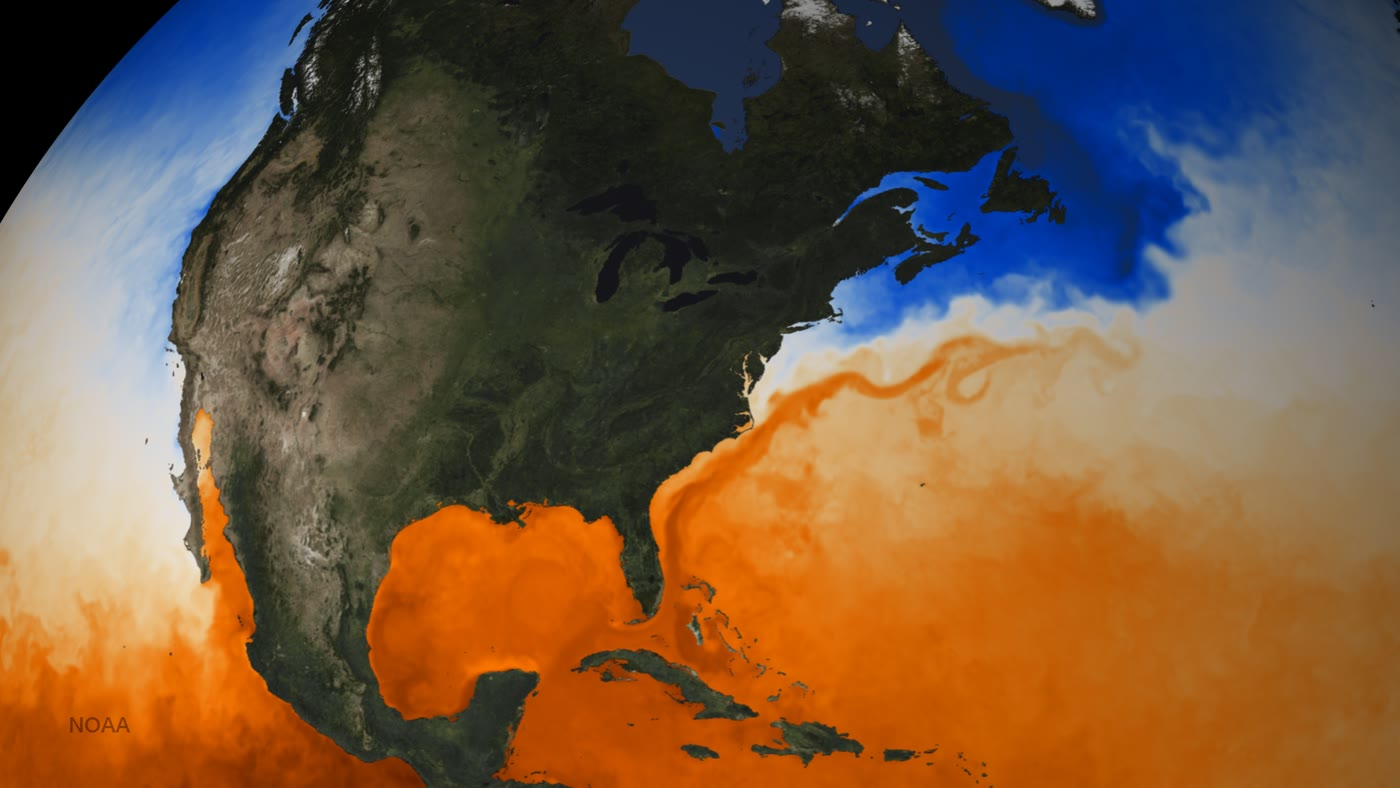
\includegraphics[width=0.85\linewidth]{images/book3/b1-gulf-stream-sst.jpg}

{\small La température de la surface de la mer autour de l'Amérique du Nord début juin 2016,
d'après des données satellitaires (eau chaude en orange, eau froide en bleu). Le Gulf Stream
quitte la côte des États-Unis en un ruban chaud et sinueux et traverse
l'Atlantique vers l'Europe~; aux mêmes \omterm{def:b1:spherical-astronomy:geographic}{latitudes}, l'eau au large de la côte Pacifique est
bien plus fraîche qu'au large de la côte Atlantique. (NOAA, NESDIS, domaine public, via
Wikimedia Commons.)}
\label{fig:b1:ocean-circulation:sst}
\end{omfigure}
% ledger: commons:gulf-stream-sst, noaa:gulf-stream-heat

\begin{recall}
Les volumes de physique donnent la force de Coriolis. Le \cref{ch:b1:atmospheric-circulation}
a écrit sa partie horizontale $-f\,\vec k\times\vec v$, avec le \omterm{def:b1:atmospheric-circulation:coriolis-parameter}{paramètre de Coriolis}
$f = 2\Omega\sin\varphi$ ($\Omega = \qty{7.292e-5}{rad.s^{-1}}$), et a trouvé les
\omterm{def:b1:atmospheric-circulation:winds}{alizés}, vents d'est entre l'équateur et environ \ang{30}, et les \omterm{def:b1:atmospheric-circulation:winds}{vents d'ouest}
au-delà~; il a aussi défini la \omterm{def:b1:atmospheric-circulation:streamfunction}{fonction de courant méridienne moyenne} d'un retournement.
Le \cref{ch:b1:fluid-envelopes-structure} a donné la \omterm{def:b1:fluid-envelopes-structure:ocean-layers}{couche de mélange} et la \omterm{def:b1:fluid-envelopes-structure:ocean-layers}{thermocline}, la
masse volumique de l'eau de mer, le \omterm{def:b1:fluid-envelopes-structure:ts-diagram}{diagramme T--S} et les \omterm{def:b1:fluid-envelopes-structure:ts-diagram}{masses d'eau} de l'Atlantique Sud,
et le \cref{ch:b1:radiation-heat-transport} le transport de chaleur vers les pôles partagé entre
l'atmosphère et l'océan. Le livre~1 a décrit les courants de surface et les grands
\omterm{def:b1:ocean-circulation:gyre}{gyres}~; le livre~2 la remontée d'eau froide le long de certaines côtes.
% ledger: earth:Trot, nos:gyres
\end{recall}

\section{Le vent et les courants de surface}\label{sec:b1:ocean-circulation:wind}

Le vent met la mer en mouvement en frottant sur elle. Sa force est répartie sur la surface, et
elle se mesure, comme une pression, par unité d'aire.

\begin{definition}[Tension du vent]\label{def:b1:ocean-circulation:wind-stress}
La \emph{tension du vent}\index{tension du vent} $\vec T$ est la force horizontale par unité
d'aire exercée par le vent sur la surface de la mer, en pascals. C'est le transfert vers le bas
de la quantité de mouvement horizontale de l'air dans l'océan, et elle pointe presque dans le sens du
vent. Sa valeur est donnée par la formule globale
\[
  T = \rho_a C_D U_{10}^2,
\]
où $\rho_a = \qty{1.3}{kg.m^{-3}}$ est la masse volumique de l'air, $U_{10}$ la vitesse du vent
à \qty{10}{m} au-dessus de la mer et $C_D$ un coefficient de traînée sans dimension.
\end{definition}
% ledger: stewart:wind-stress

Le coefficient de traînée est mesuré avec des instruments rapides qui enregistrent les fluctuations
turbulentes du vent à quelques mètres au-dessus des vagues. Pour un air de stabilité neutre,
les mesures de Yelland et Taylor donnent
\[
  1000\,C_D = 0.29 + \frac{3.1}{U_{10}} + \frac{7.7}{U_{10}^2}
  \quad (\qtyrange{3}{6}{m/s}),
  \qquad
  1000\,C_D = 0.60 + 0.071\,U_{10}
  \quad (\qtyrange{6}{26}{m/s}),
\]
avec $U_{10}$ en mètres par seconde. Un vent de \qty{10}{m/s} a $C_D =
\num{1.31e-3}$ et exerce $T = 1.3 \times \num{1.31e-3} \times 100 =
\qty{0.170}{Pa}$~; un vent de \qty{5}{m/s}, \qty{0.040}{Pa}~; un coup de vent de
\qty{20}{m/s}, \qty{1.05}{Pa}. Doubler le vent de 10 à \qty{20}{m/s}
multiplie la tension par $6.2$, non par $4$~: les mers plus agitées agrippent mieux le vent. Ces
tensions sont minuscules, un millionième de la pression atmosphérique, mais elles agissent sans
répit sur tout l'océan.
% ledger: stewart:drag-coefficient (computed in figdata/bachelor-1/ekman_hodograph.py and calc/ch29.py)

La configuration de la tension suit celle des vents. Entre les \omterm{def:b1:atmospheric-circulation:winds}{alizés} des
tropiques, soufflant vers l'ouest, et les \omterm{def:b1:atmospheric-circulation:winds}{vents d'ouest} des moyennes \omterm{def:b1:spherical-astronomy:geographic}{latitudes}, soufflant
vers l'est, l'eau de surface de chaque bassin océanique est mise en rotation.

\begin{definition}[Gyre~; gyres subtropical et subpolaire]\label{def:b1:ocean-circulation:gyre}
Un \emph{gyre}\index{gyre} est un grand système de courants océaniques en rotation remplissant un
bassin océanique. Un \emph{gyre subtropical}\index{gyre subtropical} se situe entre les \omterm{def:b1:atmospheric-circulation:winds}{alizés}
et les \omterm{def:b1:atmospheric-circulation:winds}{vents d'ouest} et tourne dans le sens horaire dans l'hémisphère Nord et dans le sens
trigonométrique dans le Sud. Un \emph{gyre subpolaire}\index{gyre subpolaire} se situe du
côté polaire des \omterm{def:b1:atmospheric-circulation:winds}{vents d'ouest} et tourne dans l'autre sens.
\end{definition}
% ledger: nos:gyre-def, nos:boundary-currents, stewart:north-atlantic

Il y a cinq \omterm{def:b1:ocean-circulation:gyre}{gyres} subtropicaux, dans l'Atlantique Nord et Sud, le Pacifique Nord et
Sud et l'océan Indien~; aucun ne chevauche l'équateur. Dans l'Atlantique
Nord, le \omterm{def:b1:ocean-circulation:gyre}{gyre subtropical} est fermé par le Gulf Stream le long de la côte des
États-Unis à l'ouest et par le courant des Canaries au large de l'Afrique à l'est~; au nord
de lui, le \omterm{def:b1:ocean-circulation:gyre}{gyre subpolaire} tourne dans le sens trigonométrique, avec le courant nord-atlantique sur son
côté sud et le courant du Labrador coulant vers le sud le long de son côté ouest. Aux basses
\omterm{def:b1:spherical-astronomy:geographic}{latitudes}, les courants équatoriaux vers l'ouest de l'Atlantique et du Pacifique sont
séparés par un contre-courant vers l'est. Les \omterm{def:b1:ocean-circulation:gyre}{gyres} ne sont pas symétriques~: chaque \omterm{def:b1:ocean-circulation:gyre}{gyre subtropical} est
fermé par un courant fort et étroit du côté ouest de son bassin et par un courant faible et
large du côté est. Autour de l'Antarctique, où aucun continent ne l'arrête,
le courant circumpolaire antarctique coule vers l'est autour du globe, entraîné par les
\omterm{def:b1:atmospheric-circulation:winds}{vents d'ouest} de l'océan Austral.
% ledger: nos:boundary-currents, stewart:north-atlantic, stewart:heat-conveyor, lien:kuroshio, donohue:acc, stewart:acc

\begin{omfigure}
\begin{tikzpicture}
\begin{axis}[ommap, width=0.98\linewidth, xtick={-180,-120,...,180}, ytick={-60,-30,0,30,60}]
% land: figdata/shared/geo.py; ledger: data:ne-land. Arrows placed by hand from the
% ledgered pattern: nos:boundary-currents, stewart:north-atlantic, lien:kuroshio,
% donohue:acc, stewart:acc
\addplot[fill=omLithAlluv, draw=black!45, line width=0.2pt, forget plot] table {figdata/out/shared-geo-land.dat};
% North Atlantic subtropical gyre (clockwise)
\addplot[omThm, line width=1.1pt, -{Stealth[length=4pt]}, smooth] coordinates {(-80,26) (-77,32) (-70,37) (-58,40) (-44,41)};
\addplot[omThm, line width=1.1pt, -{Stealth[length=4pt]}, smooth] coordinates {(-38,40) (-28,39) (-20,36)};
\addplot[omThm, line width=1.1pt, -{Stealth[length=4pt]}, smooth] coordinates {(-19,32) (-21,24) (-26,17)};
\addplot[omThm, line width=1.1pt, -{Stealth[length=4pt]}, smooth] coordinates {(-32,14) (-45,13) (-60,15)};
% North Atlantic subpolar gyre (anticlockwise)
\addplot[omDef, line width=1.1pt, -{Stealth[length=4pt]}, smooth] coordinates {(-40,47) (-28,52) (-18,57)};
\addplot[omDef, line width=1.1pt, -{Stealth[length=4pt]}, smooth] coordinates {(-24,61) (-35,62) (-44,59)};
\addplot[omDef, line width=1.1pt, -{Stealth[length=4pt]}, smooth] coordinates {(-55,59) (-56,53) (-51,47)};
% North Pacific subtropical gyre (clockwise)
\addplot[omThm, line width=1.1pt, -{Stealth[length=4pt]}, smooth] coordinates {(123,19) (125,26) (133,32) (143,36) (156,38)};
\addplot[omThm, line width=1.1pt, smooth] coordinates {(162,39) (172,40) (180,40.5)};
\addplot[omThm, line width=1.1pt, -{Stealth[length=4pt]}, smooth] coordinates {(-180,40.5) (-165,41) (-148,40)};
\addplot[omThm, line width=1.1pt, -{Stealth[length=4pt]}, smooth] coordinates {(-133,37) (-128,29) (-122,20)};
\addplot[omThm, line width=1.1pt, -{Stealth[length=4pt]}, smooth] coordinates {(-125,13) (-150,12) (-175,13)};
\addplot[omThm, line width=1.1pt, -{Stealth[length=4pt]}, smooth] coordinates {(170,13) (152,14) (135,15)};
% South Atlantic subtropical gyre (anticlockwise)
\addplot[omThm, line width=1.1pt, -{Stealth[length=4pt]}, smooth] coordinates {(2,-8) (-15,-9) (-30,-9)};
\addplot[omThm, line width=1.1pt, -{Stealth[length=4pt]}, smooth] coordinates {(-34,-14) (-39,-24) (-47,-34)};
\addplot[omThm, line width=1.1pt, -{Stealth[length=4pt]}, smooth] coordinates {(-42,-40) (-20,-40) (2,-38)};
\addplot[omThm, line width=1.1pt, -{Stealth[length=4pt]}, smooth] coordinates {(10,-31) (9,-23) (6,-15)};
% South Pacific subtropical gyre (anticlockwise)
\addplot[omThm, line width=1.1pt, -{Stealth[length=4pt]}, smooth] coordinates {(-88,-10) (-120,-11) (-160,-12)};
\addplot[omThm, line width=1.1pt, -{Stealth[length=4pt]}, smooth] coordinates {(160,-16) (157,-26) (162,-35)};
\addplot[omThm, line width=1.1pt, -{Stealth[length=4pt]}, smooth] coordinates {(-170,-40) (-140,-41) (-105,-39)};
\addplot[omThm, line width=1.1pt, -{Stealth[length=4pt]}, smooth] coordinates {(-82,-36) (-82,-27) (-85,-17)};
% Indian Ocean subtropical gyre (anticlockwise)
\addplot[omThm, line width=1.1pt, -{Stealth[length=4pt]}, smooth] coordinates {(98,-13) (80,-14) (60,-15)};
\addplot[omThm, line width=1.1pt, -{Stealth[length=4pt]}, smooth] coordinates {(47,-22) (40,-29) (33,-34)};
\addplot[omThm, line width=1.1pt, -{Stealth[length=4pt]}, smooth] coordinates {(50,-38) (75,-37) (100,-35)};
\addplot[omThm, line width=1.1pt, -{Stealth[length=4pt]}, smooth] coordinates {(108,-31) (106,-24) (102,-18)};
% Antarctic Circumpolar Current (eastward)
\addplot[omMeth, line width=1.4pt, -{Stealth[length=5pt]}, smooth] coordinates {(-62,-58) (-40,-55) (-15,-52)};
\addplot[omMeth, line width=1.4pt, -{Stealth[length=5pt]}, smooth] coordinates {(5,-52) (40,-50) (75,-50)};
\addplot[omMeth, line width=1.4pt, -{Stealth[length=5pt]}, smooth] coordinates {(95,-51) (130,-53) (165,-56)};
\addplot[omMeth, line width=1.4pt, -{Stealth[length=5pt]}, smooth] coordinates {(-170,-58) (-130,-59) (-85,-59)};
\node[font=\scriptsize, anchor=west, fill=white, fill opacity=0.8, text opacity=1, inner sep=1pt] at (axis cs:-66,31) {Gulf Stream};
\node[font=\scriptsize, anchor=west, fill=white, fill opacity=0.8, text opacity=1, inner sep=1pt] at (axis cs:-11,25) {Canaries};
\node[font=\scriptsize, anchor=east, fill=white, fill opacity=0.8, text opacity=1, inner sep=1pt] at (axis cs:-58,52) {Labrador};
\node[font=\scriptsize, anchor=west, fill=white, fill opacity=0.8, text opacity=1, inner sep=1pt] at (axis cs:142,28) {Kuroshio};
\node[font=\scriptsize, anchor=north, fill=white, fill opacity=0.8, text opacity=1, inner sep=1pt] at (axis cs:-150,9) {Nord-équatorial};
\node[font=\scriptsize, anchor=north, fill=white, fill opacity=0.8, text opacity=1, inner sep=1pt] at (axis cs:0,-62) {courant circumpolaire antarctique};
\end{axis}
\end{tikzpicture}

{\small Les \omterm{def:b1:ocean-circulation:gyre}{gyres} de l'océan de surface (flèches schématiques sur une carte des terres).
Rouge sombre~: les cinq \omterm{def:b1:ocean-circulation:gyre}{gyres} subtropicaux, dans le sens horaire dans l'hémisphère Nord et
dans le sens trigonométrique dans le Sud, chacun avec un étroit \omterm{def:b1:ocean-circulation:wbc}{courant de bord ouest}~; bleu~:
le \omterm{def:b1:ocean-circulation:gyre}{gyre subpolaire} de l'Atlantique Nord~; vert~: le courant circumpolaire antarctique.
Seuls sont nommés les courants discutés dans le texte. Les flèches montrent le sens de
l'écoulement, non sa vitesse.}
\label{fig:b1:ocean-circulation:gyres}
\end{omfigure}
% ledger: data:ne-land, nos:boundary-currents, stewart:north-atlantic, lien:kuroshio, donohue:acc

Deux traits de cette configuration demandent explication. Le premier est le sens de rotation~:
les \omterm{def:b1:atmospheric-circulation:winds}{alizés} soufflent vers l'ouest du côté équatorial d'un \omterm{def:b1:ocean-circulation:gyre}{gyre subtropical},
et pourtant les courants du \omterm{def:b1:ocean-circulation:gyre}{gyre} ne suivent pas simplement les vents, et l'eau de surface
dérive à un angle par rapport à eux. Le second est l'asymétrie~: le flux de retour d'un \omterm{def:b1:ocean-circulation:gyre}{gyre}
est écrasé contre le côté ouest de son bassin. Les deux viennent de la rotation de
la Terre.

\section{Le transport d'Ekman}\label{sec:b1:ocean-circulation:ekman}

\begin{history}[Nansen et Ekman, 1898--1905]
Pendant son expédition dans l'Arctique, Fridtjof Nansen remarqua que le vent poussait
la glace de mer non pas dans le sens du vent mais à un angle de \ang{20} à \ang{40} à sa
droite, en regardant sous le vent. Il raisonna que trois forces devaient s'équilibrer sur la glace
en mouvement~: la poussée du vent, le frottement de l'eau, et la force de Coriolis. Il
demanda au météorologue Vilhelm Bjerknes de laisser un de ses étudiants étudier
l'influence de la rotation de la Terre sur les courants entraînés par le vent. L'étudiant, Walfrid
Ekman, élabora la théorie pour sa thèse de doctorat à Uppsala, et l'étendit en
1905. Sa solution est toujours le point de départ de la théorie de l'océan
entraîné par le vent.
\end{history}
% ledger: stewart:ekman-layer, nos:ekman-spiral

\begin{definition}[Couche d'Ekman, transport d'Ekman, spirale d'Ekman]\label{def:b1:ocean-circulation:ekman}
La \emph{couche d'Ekman}\index{couche d'Ekman} est la mince couche de surface de l'océan,
épaisse d'au plus quelques centaines de mètres, dans laquelle la \omterm{def:b1:ocean-circulation:wind-stress}{tension du vent} est transmise vers le bas
par le frottement turbulent et équilibrée par la force de Coriolis. Le \emph{transport
d'Ekman}\index{transport d'Ekman} est la \omterm{def:b1:fluid-envelopes-structure:ts-diagram}{masse d'eau} que la couche porte par
seconde à travers une bande verticale large de \qty{1}{m}, de la surface jusqu'en dessous de la
couche~:
\[
  \vec M = \int_{-d}^{0} \rho\,\vec v\,\mathrm dz \quad (\unit{kg.m^{-1}.s^{-1}});
\]
divisé par la masse volumique, c'est un transport en volume par mètre, en
\unit{m^2.s^{-1}}. La \emph{spirale d'Ekman}\index{spirale d'Ekman} est la rotation et
l'affaiblissement du courant avec la profondeur dans la couche. Les transports océaniques se comptent en
\emph{sverdrups}\index{sverdrup (unité)}~: \qty{1}{\sverdrup} $=
\qty{e6}{m^3.s^{-1}}$.
\end{definition}
% ledger: stewart:ekman-layer, stewart:ekman-transport

\begin{theorem}[Transport d'Ekman]\label{thm:b1:ocean-circulation:ekman}
En régime permanent, loin des côtes, sur une eau bien plus profonde que la \omterm{def:b1:ocean-circulation:ekman}{couche d'Ekman}, le
\omterm{def:b1:ocean-circulation:ekman}{transport d'Ekman} ne dépend que de la \omterm{def:b1:ocean-circulation:wind-stress}{tension du vent} $\vec T$ et du
\omterm{def:b1:atmospheric-circulation:coriolis-parameter}{paramètre de Coriolis} $f$~:
\[
  \vec M = \frac{1}{f}\,\vec T\times\vec k,
  \qquad |\vec M| = \frac{|\vec T|}{|f|}.
\]
Il est perpendiculaire à la \omterm{def:b1:ocean-circulation:wind-stress}{tension du vent}, à sa droite dans l'hémisphère Nord
et à sa gauche dans le Sud.
\end{theorem}
% ledger: stewart:ekman-transport

\begin{proof}
Soit $\vec\tau(z)$ la tension horizontale que l'eau au-dessus du niveau $z$
exerce sur l'eau en dessous. En surface c'est la \omterm{def:b1:ocean-circulation:wind-stress}{tension du vent}, $\vec\tau(0) =
\vec T$~; sous la couche, où les courants entraînés par le vent se sont éteints, elle
s'annule, $\vec\tau(-d) = \vec 0$. Une mince tranche entre $z$ et $z + \mathrm dz$,
d'aire horizontale unité, reçoit $\vec\tau(z + \mathrm dz)$ sur sa face supérieure et
$-\vec\tau(z)$ sur sa face inférieure~: la force de frottement nette est $(\partial\vec
\tau/\partial z)\,\mathrm dz$. Sa masse est $\rho\,\mathrm dz$, et la force de
Coriolis horizontale sur elle est $-f\,\vec k\times\vec v\,\rho\,\mathrm dz$. En régime
permanent, sans variation horizontale d'un lieu à l'autre, les deux s'équilibrent~:
\[
  -f\rho\,\vec k\times\vec v + \frac{\partial\vec\tau}{\partial z} = \vec 0 .
\]
En intégrant de $-d$ à $0$,
\[
  -f\,\vec k\times\vec M + \vec\tau(0) - \vec\tau(-d) = \vec 0,
  \qquad\text{c'est-à-dire}\qquad \vec k\times\vec M = \frac{\vec T}{f}.
\]
Pour un vecteur horizontal, $\vec k\times(\vec k\times\vec M) = -\vec M$~; en prenant
$\vec k\times$ des deux membres on obtient $-\vec M = \vec k\times\vec T/f$, donc $\vec M =
\vec T\times\vec k/f$. Le vecteur $\vec T\times\vec k$ est $\vec T$ tourné de
\ang{90} dans le sens horaire vu d'en haut~: à droite du vent quand $f > 0$, à
gauche quand $f < 0$. Sa valeur est $|\vec T|$.
\end{proof}

Le résultat ne dépend pas de la façon dont le frottement agit à l'intérieur de la couche, qui est
mal connue~: seuls la tension au sommet et son annulation en bas interviennent.
Cela rend le transport bien plus robuste que les vitesses elles-mêmes. L'eau
de toute la couche, prise ensemble, se déplace à angle droit du vent, résultat qui
paraît étrange jusqu'à ce qu'on se rappelle que sur un jour ou plus la force de Coriolis a
le temps de tourner chaque courant.

\begin{example}[Le transport sous une bonne brise]\label{ex:b1:ocean-circulation:transport}
Un vent de \qty{10}{m/s} soufflant vers le nord à \ang{35}~N exerce
$T = \qty{0.170}{Pa}$. Avec $f = 2\Omega\sin\ang{35} = \qty{8.365e-5}{s^{-1}}$, le
\omterm{def:b1:ocean-circulation:ekman}{transport d'Ekman} est $0.170/(\num{8.365e-5}) = \qty{2036}{kg.m^{-1}.s^{-1}}$, vers
l'est. Avec $\rho = \qty{1027}{kg.m^{-3}}$, cela fait \qty{1.98}{m^3.s^{-1}} par
mètre mesuré à travers le transport~: à travers une ligne longue de \qty{1000}{km}, environ
\qty{2}{\sverdrup}.
\end{example}
% ledger: stewart:drag-coefficient, stewart:ekman-constants, earth:Trot (computed in calc/ch29.py)

Le théorème a été vérifié en mer. À travers \ang{11}~N dans l'Atlantique, où les
\omterm{def:b1:atmospheric-circulation:winds}{alizés} soufflent vers l'ouest, le \omterm{def:b1:ocean-circulation:ekman}{transport d'Ekman} est dirigé vers le nord~; mesuré
directement avec un profileur de courant, il a atteint
\qty[uncertainty-mode=separate]{12.0 \pm 5.5}{\sverdrup}, contre
\qty[uncertainty-mode=separate]{8.8 \pm 1.9}{\sverdrup} calculés d'après les vents
mesurés pendant la campagne et
\qty[uncertainty-mode=separate]{13.5 \pm 0.3}{\sverdrup} d'après des vents moyennés sur
de nombreuses années.
% ledger: stewart:ekman-transport

La répartition du courant avec la profondeur dans la couche dépend du
frottement. Ekman prit le modèle le plus simple, un frottement turbulent proportionnel au
cisaillement vertical du courant, $\vec\tau = \rho A_z\,\partial\vec v/\partial z$, avec
une viscosité turbulente constante $A_z$.

\begin{proposition}[La spirale d'Ekman]\label{prop:b1:ocean-circulation:spiral}
Pour une tension de vent permanente $T$ vers le nord sur un océan profond et homogène de
l'hémisphère Nord, avec une viscosité turbulente constante $A_z$, le courant à la hauteur $z
\leq 0$ est
\[
  u = V_0\,e^{az}\cos\Bigl(\frac\pi4 + az\Bigr),\qquad
  v = V_0\,e^{az}\sin\Bigl(\frac\pi4 + az\Bigr),\qquad
  a = \sqrt{\frac{f}{2A_z}},\quad V_0 = \frac{T}{\rho\sqrt{fA_z}},
\]
avec $u$ vers l'est et $v$ vers le nord. En surface le courant coule à \ang{45} à
droite du vent~; avec la profondeur il s'affaiblit comme $e^{az}$ et tourne davantage vers la
droite. À la profondeur $D_E = \pi/a$, la profondeur d'Ekman, il coule à l'opposé du courant de
surface avec $e^{-\pi} = \num{0.043}$ de sa vitesse.
\end{proposition}
\admitted
% ledger: stewart:ekman-solution

La démonstration résout les deux équations $f v + A_z u'' = 0$ et $-f u + A_z v'' =
0$ du bilan de la preuve ci-dessus~; elle se fait dans le volume de troisième année, et
l'\cref{exo:b1:ocean-circulation:10} vérifie que les formules satisfont les équations
et que la spirale porte exactement le transport du théorème. Pour employer la
spirale, il faut $A_z$, qui n'est pas mesuré directement. Ekman a rassemblé les
vitesses observées des courants de surface et a trouvé, pour $|\varphi| \geq \ang{10}$,
\[
  V_0 = \frac{0.0127\,U_{10}}{\sqrt{\sin|\varphi|}},
  \qquad\text{ce qui donne}\qquad
  D_E = \frac{7.6\,U_{10}}{\sqrt{\sin|\varphi|}},
\]
en unités SI, avec son coefficient de traînée $C_D = \num{2.6e-3}$ et $\rho_a =
\qty{1.25}{kg.m^{-3}}$. À \ang{35}~N sous un vent de \qty{10}{m/s}, $D_E =
\qty{100}{m}$ et $V_0 = \qty{0.17}{m/s}$~; la \omterm{def:b1:ocean-circulation:ekman}{couche d'Ekman} va d'environ
\qty{45}{m} sous des vents faibles aux \omterm{def:b1:spherical-astronomy:geographic}{latitudes} moyennes à \qty{300}{m} sous un coup de vent dans les
tropiques, et le courant de surface est de \qtyrange{1}{2.5}{\percent} du vent.
% ledger: stewart:ekman-constants (computed in figdata/bachelor-1/ekman_hodograph.py)

\begin{omfigure}
\begin{tikzpicture}
\begin{axis}[ompt, name=hodo, width=0.5\linewidth, axis equal image, xmin=-6, xmax=22,
  ymin=-6, ymax=17, xlabel={courant vers l'est (\unit{cm/s})}, ylabel={courant vers le nord (\unit{cm/s})},
  xtick={-5,0,5,10,15,20}, ytick={-5,0,5,10,15}]
% figdata/bachelor-1/ekman_hodograph.py; ledger: stewart:ekman-solution, stewart:ekman-constants
\addplot[black!45, line width=0.6pt] table[x expr=\thisrow{u}*100, y expr=\thisrow{v}*100] {figdata/out/bachelor-1-ekman_hodograph-tips.dat};
\addplot[omDef, line width=0.6pt, -{Stealth[length=3pt]}, quiver={u=\thisrow{u}*100, v=\thisrow{v}*100}]
  table[x expr=0, y expr=0] {figdata/out/bachelor-1-ekman_hodograph-arrows.dat};
\draw[omThm, line width=1.6pt, -{Stealth[length=6pt]}] (axis cs:-3,0) -- (axis cs:-3,14);
\node[font=\scriptsize, text=omThm, anchor=west] at (axis cs:-2.6,13) {vent};
\draw[omMeth, line width=1.6pt, -{Stealth[length=6pt]}] (axis cs:0,-3.2) -- (axis cs:16,-3.2);
\node[font=\scriptsize, text=omMeth, anchor=north] at (axis cs:8,-3.6) {transport d'Ekman};
\node[font=\scriptsize, anchor=south west] at (axis cs:11.9,11.9) {surface};
\node[font=\scriptsize, anchor=north east] at (axis cs:-0.3,-0.4) {$D_E$};
\end{axis}
\begin{axis}[ompt, at={(hodo.east)}, anchor=west, xshift=1.4cm, width=0.42\linewidth, height=6.2cm,
  xmin=-4, xmax=14, ymin=-200, ymax=0, xlabel={courant (\unit{cm/s})}, ylabel={profondeur (\unit{m})},
  yticklabel={$\pgfmathprintnumber[fixed]{\tick}$},
  legend style={font=\scriptsize, at={(0.97,0.03)}, anchor=south east, cells={anchor=west}}]
\addplot[black!40, forget plot] coordinates {(0,-200) (0,0)};
\addplot[omDef, line width=1pt] table[x expr=\thisrow{u}*100, y=z] {figdata/out/bachelor-1-ekman_hodograph-profile.dat};
\addlegendentry{vers l'est}
\addplot[omProp, line width=1pt, dashed] table[x expr=\thisrow{v}*100, y=z] {figdata/out/bachelor-1-ekman_hodograph-profile.dat};
\addlegendentry{vers le nord}
\addplot[black!50, densely dotted, forget plot] coordinates {(-4,-100.35) (14,-100.35)};
\node[font=\scriptsize, anchor=south east] at (axis cs:13.8,-100.35) {$D_E = \qty{100}{m}$};
\end{axis}
\end{tikzpicture}

{\small La \omterm{def:b1:ocean-circulation:ekman}{spirale d'Ekman} sous un vent de \qty{10}{m/s} soufflant vers le nord à
\ang{35}~N, avec les constantes d'Ekman. À gauche~: le courant vu d'en haut en
surface et à chaque dixième de la profondeur d'Ekman $D_E$ jusqu'à $D_E$ (flèches bleues), la
courbe grise joignant leurs pointes~; le courant de surface est à \ang{45} à droite du
vent, les plus profonds sont plus faibles et tournés davantage à droite. Le transport de toute la
couche (vert~; direction seule) est à \ang{90} à droite du vent.
À droite~: les deux composantes en fonction de la profondeur.}
\label{fig:b1:ocean-circulation:spiral}
\end{omfigure}
% ledger: stewart:ekman-solution, stewart:ekman-constants

La spirale est une idéalisation. Des mesures de courantomètres sur des mouillages et
de 1503 dériveurs suivis dans le Pacifique entre 1987 et 1994 montrent que, moyenné
sur de nombreux jours, l'écoulement s'accorde remarquablement bien avec la théorie d'Ekman~: la profondeur de la
couche est presque la sienne, $7.12\,U_{10}/\sqrt{\sin|\varphi|}$~; le courant de surface est
environ la moitié de sa valeur~; l'angle entre le vent et l'écoulement de surface est proche de
\ang{45} aux \omterm{def:b1:spherical-astronomy:geographic}{latitudes} moyennes~; et le transport est à \ang{90} à droite du vent.
Sur quelques heures, le tableau est brouillé par les oscillations d'inertie, et l'équilibre
demande que le vent souffle régulièrement pendant un jour ou deux pour s'établir.
% ledger: stewart:ekman-observed

\section{La remontée d'eaux profondes et le pompage d'Ekman}\label{sec:b1:ocean-circulation:upwelling}

Là où le \omterm{def:b1:ocean-circulation:ekman}{transport d'Ekman} n'est pas le même partout, l'eau s'accumule en certains endroits
et est emportée d'autres~; la différence est compensée par un mouvement vertical.

\begin{definition}[Remontée d'eaux, plongée d'eaux, remontée côtière]\label{def:b1:ocean-circulation:upwelling}
La \emph{remontée d'eaux}\index{remontee d'eaux@remontée d'eaux} (\textit{upwelling}) est la montée d'eau d'en dessous dans la couche de surface
de l'océan, pour remplacer l'eau de surface emportée~; la \emph{plongée d'eaux}%
\index{plongee d'eaux@plongée d'eaux} est l'enfoncement de l'eau de surface là où elle s'accumule.
La \emph{remontée côtière}\index{remontee cotiere@remontée côtière} se produit là où un vent soufflant le long
d'une côte entraîne un \omterm{def:b1:ocean-circulation:ekman}{transport d'Ekman} qui s'éloigne du rivage~: dans l'hémisphère Nord,
un vent ayant la côte à sa gauche.
\end{definition}
% ledger: noaa:upwelling, stewart:upwelling

\begin{proposition}[Remontée côtière]\label{prop:b1:ocean-circulation:coastal}
Le long d'une côte rectiligne de longueur $L$, une tension de vent de composante $T_\parallel$
le long de la côte, dirigée de sorte que le \omterm{def:b1:ocean-circulation:ekman}{transport d'Ekman} pointe vers le large, fait remonter
d'en dessous de la \omterm{def:b1:ocean-circulation:ekman}{couche d'Ekman} le volume
\[
  Q = \frac{T_\parallel\,L}{\rho\,|f|}
\]
par seconde.
\end{proposition}
% ledger: stewart:upwelling, stewart:ekman-transport

\begin{proof}
D'après le \cref{thm:b1:ocean-circulation:ekman}, le transport à travers la côte est
produit par la composante de la tension le long d'elle, et a pour valeur
$T_\parallel/|f|$ par mètre de côte~; il emporte $T_\parallel L/(\rho|f|)$ mètres
cubes par seconde vers le large à travers une ligne parallèle à la côte. À la côte elle-même
aucune eau ne peut passer. En régime permanent la \omterm{def:b1:fluid-envelopes-structure:ts-diagram}{masse d'eau} entre la côte et cette
ligne ne change pas~: l'eau qui part en surface doit entrer par en dessous,
à travers la base de la \omterm{def:b1:ocean-circulation:ekman}{couche d'Ekman}.
\end{proof}

\begin{omfigure}
\begin{tikzpicture}[>={Stealth[length=2.2mm]}, font=\scriptsize]
% plan view
\begin{scope}
  \fill[omSea] (0,0) rectangle (3.2,4.2);
  \fill[omLithAlluv] (3.2,0) -- (3.2,4.2) -- (4.2,4.2) -- (4.2,0) -- cycle;
  \draw[black!60] (3.2,0) -- (3.2,4.2);
  \node[rotate=90] at (3.75,2.1) {terre};
  \draw[omThm, line width=1.4pt, ->] (2.5,3.6) -- (2.5,1.4);
  \node[omThm, anchor=east] at (2.42,2.6) {vent};
  \draw[omMeth, line width=1.4pt, ->] (2.2,0.9) -- (0.4,0.9);
  \node[omMeth, anchor=south, align=center] at (1.3,0.95) {transport\\d'Ekman};
  \draw[line width=0.8pt, ->] (0.4,3.3) -- (0.4,4.0) node[above, inner sep=1pt] {N};
  \node[anchor=north] at (2.1,-0.1) {vue en plan};
\end{scope}
% cross-section, looking north: west on the left, east on the right
\begin{scope}[xshift=5.2cm]
  \fill[omSea] (0,-3.6) rectangle (8.0,0);
  \fill[omSea!70!blue!35] (0,-0.9) rectangle (8.0,0);
  \fill[omLithAlluv] (8.6,0.5) -- (8.6,-3.6) -- (5.4,-3.6) -- (7.2,-1.2) -- (8.0,0) -- (8.3,0.3) -- cycle;
  \draw[black!60] (5.4,-3.6) -- (7.2,-1.2) -- (8.0,0) -- (8.3,0.3);
  \draw[black!50] (0,0) -- (8.0,0);
  % isotherms rising towards the coast
  \foreach \y/\t in {-1.5/{chaud}, -2.2/{}, -2.9/{froid}} {
    \draw[omDef, densely dashed] (0,\y) .. controls (3.5,\y) and (5.6,\y+0.7) .. (6.7,\y+1.15);
  }
  \node[anchor=west, text=omDef] at (0.05,-1.85) {isothermes};
  \draw[omMeth, line width=1.4pt, ->] (6.0,-0.45) -- (1.0,-0.45);
  \node[omMeth, anchor=south] at (3.5,-0.42) {transport d'Ekman, vers le large};
  \node[anchor=north west] at (0.05,-0.92) {couche d'Ekman};
  \draw[omThm, line width=1.2pt, ->] (4.6,-2.9) .. controls (6.2,-2.6) and (6.8,-1.6) .. (7.25,-0.55);
  \node[omThm, anchor=east, align=right, fill=omSea, inner sep=1pt] at (4.5,-2.7) {l'eau froide, riche en nutriments,\\remonte};
  \draw[omThm, line width=1pt] (6.3,0.85) circle (0.17);
  \fill[omThm] (6.3,0.85) circle (0.05);
  \node[omThm, anchor=east] at (6.05,0.85) {vent vers l'observateur (sud)};
  \fill[black!15] (7.5,1.1) ellipse (0.55 and 0.18);
  \fill[black!15] (8.0,1.2) ellipse (0.45 and 0.16);
  \node[anchor=south] at (7.8,1.3) {brouillard, nuages bas};
  \node[anchor=north] at (0.2,-3.65) {O};
  \node[anchor=north] at (8.4,-3.65) {E};
  \node[anchor=north] at (4.2,-3.65) {coupe, vers le nord};
\end{scope}
\end{tikzpicture}

{\small \omterm{def:b1:ocean-circulation:upwelling}{Remontée côtière} sur le côté oriental d'un océan de l'hémisphère
Nord (schématique, profondeurs hors échelle). À gauche~: un vent soufflant vers le sud
le long d'une côte orientée nord--sud, la terre étant à l'est~; le \omterm{def:b1:ocean-circulation:ekman}{transport
d'Ekman} est à \ang{90} à droite du vent, vers le large. À droite~: la même scène vue en
coupe verticale~; l'eau emportée vers le large dans la \omterm{def:b1:ocean-circulation:ekman}{couche d'Ekman} est remplacée par
en dessous, les isothermes montent vers la côte, et l'eau froide en surface refroidit
l'air au-dessus d'elle.}
\label{fig:b1:ocean-circulation:upwelling}
\end{omfigure}
% ledger: stewart:upwelling, noaa:upwelling

Au large de la Californie, où les vents d'été soufflent vers le sud le long de la côte,
la situation est exactement celle de la figure. L'eau
remontée vient de sous la \omterm{def:b1:fluid-envelopes-structure:ocean-layers}{couche de mélange}~: elle est plus froide que l'eau de surface, et
plus riche en nutriments. Les nutriments nourrissent le phytoplancton, qui nourrit le
zooplancton et les poissons~: les régions de remontée au large du Pérou, de la Californie, de la Somalie,
du Maroc et de la Namibie soutiennent certaines des principales pêcheries du monde. L'eau froide
change aussi le temps sur la côte~: l'air qui la traverse est refroidi par en dessous et
devient stratifié de façon stable, et ces côtes ont tendance à avoir du brouillard, des stratus bas,
peu de convection et peu de pluie. La photographie qui ouvre le chapitre montre le
contraste~: l'eau froide au large de la côte Pacifique de l'Amérique du Nord, l'eau chaude au large de
la côte Atlantique aux mêmes \omterm{def:b1:spherical-astronomy:geographic}{latitudes}.
% ledger: stewart:upwelling, noaa:upwelling, noaa:gulf-stream-heat

La \omterm{def:b1:ocean-circulation:upwelling}{remontée d'eaux} n'a pas besoin d'une côte. Le long de l'équateur, les \omterm{def:b1:atmospheric-circulation:winds}{alizés} soufflent vers
l'ouest des deux côtés~; juste au nord de l'équateur leur \omterm{def:b1:ocean-circulation:ekman}{transport d'Ekman} est à droite,
vers le nord, et juste au sud de lui à gauche, vers le sud. L'eau de surface diverge
de l'équateur, et l'eau froide monte le long de lui. En plein océan, partout où le
transport varie d'un lieu à l'autre, le même bilan de masse s'applique.

\begin{proposition}[Pompage d'Ekman]\label{prop:b1:ocean-circulation:pumping}
Là où le \omterm{def:b1:ocean-circulation:ekman}{transport d'Ekman} $\vec M$ change d'un lieu à l'autre, l'eau traverse la
base de la \omterm{def:b1:ocean-circulation:ekman}{couche d'Ekman} avec la vitesse ascendante
\[
  w_E = \frac{1}{\rho}\Bigl(\frac{\partial M_x}{\partial x} + \frac{\partial M_y}{\partial y}\Bigr):
\]
l'eau monte là où les transports divergent et descend là où ils convergent.
\end{proposition}
% ledger: stewart:upwelling

\begin{proof}
Prenons une colonne de la \omterm{def:b1:ocean-circulation:ekman}{couche d'Ekman} avec une petite base rectangulaire $\mathrm dx\,\mathrm
dy$. À travers ses côtés ouest et est, la couche apporte $M_x(x)\,\mathrm dy$
et emporte $M_x(x + \mathrm dx)\,\mathrm dy$ kilogrammes par seconde~; le flux sortant net est
$(\partial M_x/\partial x)\,\mathrm dx\,\mathrm dy$, et de même
$(\partial M_y/\partial y)\,\mathrm dx\,\mathrm dy$ à travers les côtés sud et
nord. La surface ne peut monter dans l'air, et en régime permanent la masse
de la colonne est constante~: le flux sortant net est fourni par de l'eau entrant par
sa base, $\rho w_E\,\mathrm dx\,\mathrm dy$.
\end{proof}

Dans un \omterm{def:b1:ocean-circulation:gyre}{gyre subtropical} les \omterm{def:b1:atmospheric-circulation:winds}{alizés} du côté équatorial entraînent un \omterm{def:b1:ocean-circulation:ekman}{transport
d'Ekman} vers le pôle, et les \omterm{def:b1:atmospheric-circulation:winds}{vents d'ouest} du côté polaire un transport
vers l'équateur~: les deux convergent, et l'eau de surface est pompée vers le bas. Prenons,
à titre d'illustration, une tension de \qty{0.08}{Pa} vers l'ouest à \ang{15}~N et de
\qty{0.10}{Pa} vers l'est à \ang{45}~N. Les transports sont
$0.08/f(\ang{15}) = \qty{2119}{kg.m^{-1}.s^{-1}}$ vers le nord et $0.10/f(\ang{45}) =
\qty{970}{kg.m^{-1}.s^{-1}}$ vers le sud. Leur convergence sur les \qty{3340}{km}
entre les deux \omterm{def:b1:spherical-astronomy:geographic}{latitudes} donne une vitesse descendante moyenne de
$(2119 + 970)/(1027 \times \num{3.34e6}) = \qty{9.0e-7}{m/s}$, environ \qty{28}{m}
par an. Ce lent enfoncement accumule de l'eau chaude de surface dans le \omterm{def:b1:ocean-circulation:gyre}{gyre} et approfondit sa
\omterm{def:b1:fluid-envelopes-structure:ocean-layers}{thermocline}~; les \omterm{def:b1:ocean-circulation:gyre}{gyres subpolaires}, sous des transports divergents, sont pompés vers le haut. La
façon dont l'intérieur de l'océan répond à ce pompage, le bilan de Sverdrup, est un
sujet du volume de troisième année. Autour de l'Antarctique, les \omterm{def:b1:ocean-circulation:ekman}{transports d'Ekman} divergent au sud
du maximum des \omterm{def:b1:atmospheric-circulation:winds}{vents d'ouest}, près de \ang{50}~S, et amènent l'Eau profonde circumpolaire
jusqu'à la surface~; ils convergent au nord de lui et poussent l'Eau intermédiaire antarctique
vers le bas.
% ledger: stewart:upwelling, stewart:acc (illustrative stresses; computed in calc/ch29.py)

\section{Les courants de bord ouest}\label{sec:b1:ocean-circulation:wbc}

\begin{definition}[Courant de bord ouest]\label{def:b1:ocean-circulation:wbc}
Un \emph{courant de bord ouest}\index{courant de bord ouest} est le courant rapide et
étroit, dirigé vers le pôle, qui longe le côté ouest d'un bassin océanique et
ferme son \omterm{def:b1:ocean-circulation:gyre}{gyre subtropical}. Le courant qui ferme le \omterm{def:b1:ocean-circulation:gyre}{gyre} du côté est,
un courant de bord est, est faible, large et coule vers l'équateur.
\end{definition}
% ledger: nos:boundary-currents, lien:kuroshio

Le Gulf Stream est le \omterm{def:b1:ocean-circulation:wbc}{courant de bord ouest} de l'Atlantique Nord. Il sort
du golfe du Mexique, quitte celui-ci par le détroit de Floride, et longe la côte des
États-Unis avant de tourner à travers l'océan vers l'Europe. Sa vitesse moyenne
est d'environ \qty{6.4}{km/h}, \qty{1.8}{m/s}, atteignant \qty{9}{km/h} près de la
surface. À travers le détroit de Floride il porte
\qty[uncertainty-mode=separate]{31.7 \pm 2.2}{\sverdrup} (moyenne et écart-type
des valeurs mensuelles, 2004--2024, mesurées surtout avec un câble sous-marin
électromagnétique), et son transport croît
vers l'aval, jusqu'à environ \qty{150}{\sverdrup} près de \ang{40}~N, à mesure qu'il rassemble l'eau
d'une recirculation au sud de lui. Son tracé fait des méandres, et les méandres se détachent en anneaux
d'environ un degré de large~; l'énergie cinétique de ces tourbillons est 8 à 37 fois celle de
l'écoulement moyen. Dans le Pacifique Nord, le Kuroshio joue le même rôle~: il naît
à l'est de Luçon, aux Philippines, où le courant nord-équatorial se divise, longe la
côte est de Taïwan et le sud du Japon, et croît aussi en allant vers le nord, d'environ
\qty{16}{\sverdrup} à \ang{18.75}~N.
% ledger: nos:gulf-stream, nos:boundary-currents, rapid:transports, stewart:north-atlantic, lien:kuroshio

\begin{history}[Stommel 1948]
En 1948 Henry Stommel prit l'océan le plus simple qu'il pût imaginer~: un bassin rectangulaire
de profondeur uniforme, rempli d'une eau de masse volumique uniforme, entraîné par un vent soufflant
vers l'ouest dans sa moitié sud et vers l'est dans sa moitié nord, et
ralenti par un frottement au fond proportionnel à la vitesse. Sans rotation,
ou avec une rotation uniforme, le \omterm{def:b1:ocean-circulation:gyre}{gyre} sortait symétrique, sans \omterm{def:b1:ocean-circulation:wbc}{courant de bord
ouest}. Ce n'est que lorsqu'il laissa le \omterm{def:b1:atmospheric-circulation:coriolis-parameter}{paramètre de Coriolis} croître vers le nord que les
lignes de courant se serrèrent contre le bord ouest. Il suggéra que c'était la principale
raison du Gulf Stream et des autres courants intenses des océans~;
l'explication, en termes de rotation donnée à l'eau par le vent et retirée au
bord ouest, relève du volume de troisième année.
\end{history}
% ledger: stommel:1948, stewart:stommel

\begin{omfigure}
\begin{tikzpicture}
\begin{groupplot}[group style={group size=2 by 2, horizontal sep=0.9cm, vertical sep=1.1cm,
    xlabels at=edge bottom, ylabels at=edge left},
  ompt, width=0.5\linewidth, xmin=0, xmax=1.5, xtick={0,0.5,1,1.5},
  tick label style={font=\scriptsize}, every axis label/.append style={font=\scriptsize}]
% figdata/bachelor-1/stommel_gyre.py; ledger: stommel:1948, stewart:stommel
\nextgroupplot[axis equal image, ymin=0, ymax=1, ytick={0,0.5,1}, ylabel={nord},
  title={\scriptsize rotation uniforme}]
\addplot[omThm, line width=0.7pt, unbounded coords=jump] table {figdata/out/bachelor-1-stommel_gyre-seg-uniform.dat};
\nextgroupplot[axis equal image, ymin=0, ymax=1, ytick={0,0.5,1}, yticklabels={},
  title={\scriptsize paramètre de Coriolis croissant vers le nord}]
\addplot[omThm, line width=0.7pt, unbounded coords=jump] table {figdata/out/bachelor-1-stommel_gyre-seg-beta.dat};
\nextgroupplot[height=3.6cm, ymin=-1.1, ymax=1.1, ytick={-1,0,1}, xlabel={est}, ylabel={courant vers le nord}]
\addplot[black!40] coordinates {(0,0) (1.5,0)};
\addplot[omDef, line width=0.9pt] table[x=x, y=v] {figdata/out/bachelor-1-stommel_gyre-vsec-uniform.dat};
\nextgroupplot[height=3.6cm, ymin=-1.1, ymax=1.1, ytick={-1,0,1}, yticklabels={}, xlabel={est}]
\addplot[black!40] coordinates {(0,0) (1.5,0)};
\addplot[omDef, line width=0.9pt] table[x=x, y=v] {figdata/out/bachelor-1-stommel_gyre-vsec-beta.dat};
\end{groupplot}
\end{tikzpicture}

{\small Le \omterm{def:b1:ocean-circulation:gyre}{gyre} de Stommel, calculé dans un bassin 1.5 fois plus large que long, avec le vent
vers l'ouest au sud et vers l'est au nord. En haut~: les
lignes de courant (l'écoulement tourne dans le sens horaire le long d'elles, à 10, 30, 50, 70 et
\qty{90}{\percent} de la plus grande valeur). En bas~: le courant vers le nord à travers le
milieu du bassin, divisé par sa plus grande valeur. Avec une rotation uniforme (à gauche)
le \omterm{def:b1:ocean-circulation:gyre}{gyre} est symétrique~; quand le \omterm{def:b1:atmospheric-circulation:coriolis-parameter}{paramètre de Coriolis} croît vers le nord
(à droite), l'écoulement de retour vers le nord est comprimé en un courant étroit et rapide contre
le bord ouest, et la lente dérive vers le sud remplit le reste du bassin.
Le frottement et le taux de croissance de $f$ sont des valeurs d'exercice.}
\label{fig:b1:ocean-circulation:stommel}
\end{omfigure}
% ledger: stommel:1948, stewart:stommel

Dans le \omterm{def:b1:ocean-circulation:gyre}{gyre} calculé de la figure ci-dessus, le courant vers le nord le plus rapide au
bord ouest est 37 fois la dérive vers le sud de l'intérieur. Dans un océan réel
la dérive intérieure est trop lente pour être mesurée directement face aux tourbillons~;
l'\cref{exo:b1:ocean-circulation:11} estime les deux vitesses.
Dans l'Atlantique Nord, la théorie de l'intérieur prédit un \omterm{def:b1:ocean-circulation:wbc}{courant de bord ouest}
d'environ \qty{30}{\sverdrup}, le plus grand près de \ang{28}~N, proche du transport
mesuré dans le détroit de Floride~; le flux bien plus grand au large du cap Hatteras et près de
\ang{40}~N est alimenté par une recirculation de l'eau propre du Gulf Stream, au sud de lui.
% ledger: stewart:north-atlantic (computed in figdata/bachelor-1/stommel_gyre.py)

\section{La circulation méridienne de retournement}\label{sec:b1:ocean-circulation:moc}

Le vent met en mouvement les quelques centaines de mètres supérieurs de l'océan. En dessous, l'eau de
l'abysse est renouvelée par une lente circulation qui démarre en quelques endroits des océans
polaires, où l'eau de surface devient assez dense pour couler jusqu'au fond.

\begin{definition}[Circulation méridienne de retournement~; circulation thermohaline~; formation d'eau profonde]\label{def:b1:ocean-circulation:moc}
La \emph{circulation méridienne de retournement}\index{circulation meridienne de retournement@circulation méridienne de retournement} (AMOC dans l'Atlantique) d'un bassin océanique est sa
circulation dans le plan latitude--profondeur,
obtenue en additionnant l'écoulement vers le nord sur toute la largeur du bassin. À une
\omterm{def:b1:spherical-astronomy:geographic}{latitude} donnée son intensité est le maximum de la fonction de courant de retournement, le
transport vers le nord intégré de la surface jusqu'à une profondeur donnée, en
\omterm{def:b1:ocean-circulation:ekman}{sverdrups}. L'ancien nom de \emph{circulation
thermohaline}\index{circulation thermohaline} décrit la même circulation profonde comme
entraînée par des différences de température et de salinité. La \emph{formation d'eau
profonde}\index{formation d'eau profonde} est l'enfoncement d'eau de surface, rendue dense
par le refroidissement et par le sel laissé derrière quand la glace de mer se forme, jusqu'à des profondeurs intermédiaires ou abyssales.
\end{definition}
% ledger: stewart:moc-term, rapid:transports, nos:sea-ice-salt, nos:conveyor

Le nom «~thermohaline~» a presque disparu de la littérature de recherche, car
la circulation profonde n'est pas entraînée par les seules différences de masse volumique~: les vents qui
font monter l'eau profonde dans l'océan Austral, et le mélange qui la soulève ailleurs,
sont nécessaires pour fermer la boucle. La fonction de courant de retournement est l'homologue océanique
de la fonction de courant de la \cref{def:b1:atmospheric-circulation:streamfunction},
écrite en volume plutôt qu'en masse.
% ledger: stewart:moc-term, stewart:acc

L'eau profonde se forme là où l'eau de surface est à la fois froide et salée. En hiver, l'eau de
surface de l'extrême Atlantique Nord cède sa chaleur à l'atmosphère et devient
froide, salée et assez dense pour couler dans les mers du Groenland et de Norvège, et, comme l'a noté
le \cref{ch:b1:fluid-envelopes-structure}, dans la mer du Labrador~: c'est la
source de l'Eau profonde nord-atlantique, qui se déplace vers le sud à des profondeurs voisines de
\qty{2000}{m}. Autour de l'Antarctique, dans les mers peu profondes de
Weddell et de Ross, la congélation hivernale de la mer laisse son sel dans l'eau
sous la glace et produit l'eau la plus froide et la plus salée de l'océan~; elle s'écoule
des plateaux continentaux, se mélange à l'eau profonde qu'elle rencontre, et s'étale le long
du fond marin sous le nom d'Eau de fond antarctique, \qtyrange{8}{10}{\sverdrup} de celle-ci. Entre
elles, l'Eau intermédiaire antarctique coule près du front polaire de l'océan Austral
et s'étale vers le nord près de \qty{1000}{m}, et l'eau chaude et salée qui quitte la
Méditerranée s'étale à travers l'Atlantique Nord à des profondeurs intermédiaires. Toutes
ces eaux peuvent être suivies par leur température et leur salinité, comme l'a montré la
\cref{met:b1:fluid-envelopes-structure:ts}.
% ledger: stewart:heat-conveyor, stewart:deep-circulation, stewart:acc, nos:sea-ice-salt

\begin{omfigure}
\begin{tikzpicture}[>={Stealth[length=2.2mm]}, font=\scriptsize, x=0.085cm, y=-0.66cm]
% schematic; latitudes in degrees (x), depths in km (y). ledger: stewart:deep-circulation,
% stewart:acc, stewart:heat-conveyor, rapid:transports
\fill[omSea] (-70,0) rectangle (70,6);
\fill[omLithAlluv] (-78,6.5) -- (-78,-0.3) -- (-72,-0.3) -- (-70,0.6) -- (-66,5.6) -- (-60,6) -- (66,6) -- (68,1.0) -- (70,0.4) -- (78,0.4) -- (78,6.5) -- cycle;
\draw[black!60] (-72,-0.3) -- (-70,0.6) -- (-66,5.6) -- (-60,6) -- (66,6) -- (68,1.0) -- (70,0.4);
\foreach \d in {0,1,...,6} { \draw[black!50] (-80,\d) -- (-81.5,\d) node[left] {\d}; }
\node[rotate=90] at (-92,3) {profondeur (\unit{km})};
\foreach \l/\t in {-60/60\,S, -30/30\,S, 0/0, 30/30\,N, 60/60\,N} { \draw[black!50] (\l,6.5) -- (\l,6.65) node[below] {\t}; }
% upper limb, northward
\draw[omThm, line width=1.5pt, ->] (-40,0.3) -- (55,0.3);
\node[omThm, anchor=north] at (-5,0.36) {eau chaude supérieure, vers le nord};
% sinking in the north
\draw[omThm!60!omDef, line width=1.5pt, ->] (60,0.4) .. controls (64,0.8) and (64,1.6) .. (60,2.0);
\node[anchor=west, align=left] at (63,-0.55) {mers du Groenland\\et de Norvège};
% NADW southward
\draw[omDef, line width=1.5pt, ->] (58,2.2) -- (-48,2.2);
\node[omDef, anchor=north] at (-15,2.25) {Eau profonde nord-atlantique, vers le sud};
% lower NADW, southward (the 3000-5000 m layer at 26 N)
\draw[omDef, line width=1.5pt, ->] (62,4.1) -- (-46,4.1);
\node[omDef, anchor=north] at (-15,4.15) {Eau profonde nord-atlantique inférieure, vers le sud};
% Southern Ocean upwelling
\draw[omDef, line width=1.5pt, ->] (-50,2.1) .. controls (-56,1.7) and (-58,0.8) .. (-56,0.25);
\node[anchor=west, align=left] at (-49.5,1.6) {remontée\\au sud de 50\,S};
% AAIW
\draw[omMeth, line width=1.2pt, ->] (-47,0.3) .. controls (-44,1.1) and (-38,1.3) .. (20,1.3);
\node[omMeth, anchor=north, font=\scriptsize] at (2.5,1.35) {Eau intermédiaire antarctique};
% AABW
\draw[omProp, line width=1.5pt, ->] (-69,1.0) .. controls (-66,4.4) and (-62,5.6) .. (-55,5.65) -- (30,5.65);
\node[omProp, anchor=south] at (-5,5.65) {Eau de fond antarctique, vers le nord};
\node[anchor=south] at (-72,-0.35) {mer de Weddell};
% RAPID line at 26 N
\draw[black, densely dashed] (26,0) -- (26,6);
\node[anchor=west, fill=omSea, inner sep=1pt] at (27,0.75) {$+16.6$};
\node[anchor=west, fill=omSea, inner sep=1pt] at (27,1.75) {$-12.0$};
\node[anchor=west, fill=omSea, inner sep=1pt] at (27,3.55) {$-5.9$};
\node[anchor=south] at (26,-0.05) {\ang{26} N};
\end{tikzpicture}

{\small La circulation de retournement de l'Atlantique en coupe méridienne
(schématique, profondeur exagérée). L'eau chaude supérieure coule vers le nord, cède sa chaleur à
l'atmosphère et s'enfonce dans les mers du Groenland et de Norvège~; l'Eau profonde nord-atlantique
repart vers le sud à des profondeurs de quelques kilomètres et est ramenée au sud de \ang{50}~S par
la divergence d'Ekman sous les \omterm{def:b1:atmospheric-circulation:winds}{vents d'ouest}. L'Eau intermédiaire antarctique s'étale
vers le nord au-dessus d'elle, l'Eau de fond antarctique le long du fond, sous l'Eau profonde nord-atlantique
inférieure. Nombres à \ang{26}~N~: transports moyens
en \omterm{def:b1:ocean-circulation:ekman}{sverdrups} mesurés par le réseau de mouillages, 2004--2024, positifs vers le nord,
pour les couches 0--\qty{800}{m}, \qtyrange{1100}{3000}{m} et
\qtyrange{3000}{5000}{m}.}
\label{fig:b1:ocean-circulation:moc}
\end{omfigure}
% ledger: stewart:deep-circulation, stewart:acc, stewart:heat-conveyor, rapid:transports

La force du retournement de l'Atlantique est mesurée en continu depuis 2004
le long de \ang{26.5}~N, entre la Floride et l'Afrique. Trois pièces s'additionnent~: le Gulf
Stream à travers le détroit de Floride, \qty{31.7}{\sverdrup} vers le nord~; le \omterm{def:b1:ocean-circulation:ekman}{transport
d'Ekman} calculé d'après la \omterm{def:b1:ocean-circulation:wind-stress}{tension du vent}, \qty{3.5}{\sverdrup} vers le nord~; et
l'écoulement de l'eau supérieure à travers l'océan ouvert, mesuré par des mouillages qui enregistrent
température, salinité et pression de la surface au fond marin près des deux
bords et de part et d'autre de la dorsale médio-atlantique, \qty{17.9}{\sverdrup}
vers le sud. Leur somme, l'écoulement vers le nord de l'eau supérieure
à travers tout l'océan, est le retournement~: sa moyenne d'avril 2004 à novembre
2024 est de \qty[uncertainty-mode=separate]{17.1 \pm 3.2}{\sverdrup}, le maximum de la
fonction de courant se situant en général près de \qty{1100}{m}. En dessous, l'Eau profonde nord-atlantique
supérieure porte \qty{12.0}{\sverdrup} vers le sud entre 1100 et \qty{3000}{m}, et
l'inférieure, \qty{5.9}{\sverdrup} entre 3000 et \qty{5000}{m}. Le réseau a montré que le
retournement varie d'un jour à l'autre et d'une année à l'autre bien plus que prévu,
surtout sous l'influence du vent~; après un fort creux en 2010--2011 il est resté
plus faible, et sur de courtes périodes il peut même s'inverser.
% ledger: rapid:transports, rapid:home

\begin{inthelab}[Mesurer l'océan profond]
L'océan profond se mesure à partir de mouillages et de flotteurs plutôt que de navires seuls. Un
mouillage est une ligne ancrée, allant du fond marin vers la surface,
portant des instruments qui enregistrent température, salinité, pression ou courant jusqu'à ce qu'un
navire les récupère~; une ligne de tels mouillages à travers un océan, avec un
câble électromagnétique à travers le détroit de Floride et les vents vus depuis les
satellites, donne le retournement à \ang{26.5}~N. Le
réseau Argo maintient près de \num{4000} flotteurs profileurs dans l'océan~: chacun dérive en
profondeur, puis remonte à la surface en mesurant température, salinité et pression
en chemin, et transmet son profil par satellite environ tous les dix jours. Les flotteurs standards
profilent jusqu'à \qty{2000}{m}~; les flotteurs de Deep Argo, comme celui de la
photographie ci-dessous, descendent jusqu'à \qty{6000}{m}. En 25 ans la flotte a recueilli
quelque trois millions de profils.
\end{inthelab}
% ledger: rapid:transports, noaa:argo-25, argo:fleet

\begin{omfigure}
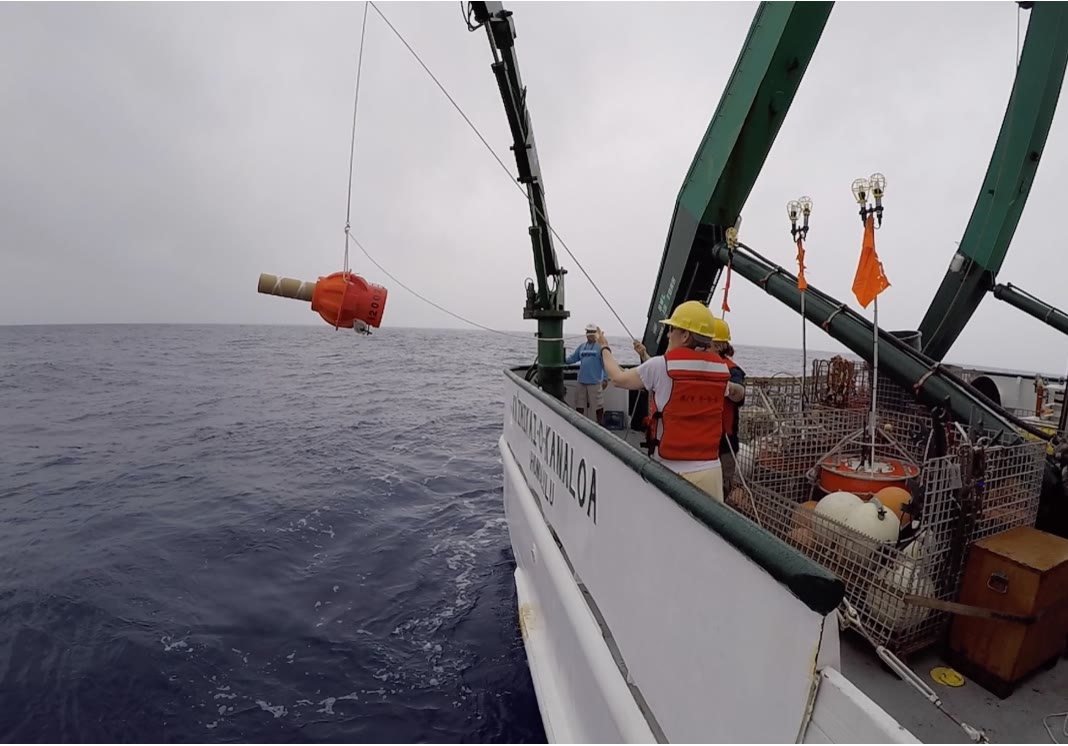
\includegraphics[width=0.6\linewidth]{images/book3/b1-deep-float.jpg}

{\small Un flotteur profileur d'océan profond (l'instrument orange suspendu à la grue)
descendu d'un navire de recherche en 2018~; une fois largué, il s'enfonce jusqu'à sa
profondeur de travail et remonte à intervalles réguliers pour envoyer ses données. (Photographe
inconnu de la NOAA, domaine public, via Wikimedia Commons.)}
\label{fig:b1:ocean-circulation:float}
\end{omfigure}
% ledger: commons:deep-solo, noaa:argo-25

Le retournement porte de la chaleur. L'eau qui va vers le nord chaude et revient froide
a cédé de la chaleur à l'atmosphère du nord.

\begin{proposition}[Chaleur portée par un retournement]\label{prop:b1:ocean-circulation:heat}
Si un transport en volume $Q$ traverse une \omterm{def:b1:spherical-astronomy:geographic}{latitude} vers le nord à la \omterm{def:b1:fluid-envelopes-structure:potential-temperature}{température potentielle}
$\theta_1$ et revient vers le sud à $\theta_2$, sans transport net de masse, le
retournement porte vers le nord le flux de chaleur
\[
  H = \rho c_p\,Q\,(\theta_1 - \theta_2),
\]
où $c_p$ est la capacité thermique massique de l'eau de mer.
\end{proposition}
% ledger: teos10:cp0

\begin{proof}
Chaque seconde, la masse $\rho Q$ traverse vers le nord en portant le contenu de chaleur $\rho Q
c_p\theta_1$, compté à partir d'un zéro de température arbitraire, et la même masse
traverse vers le sud en portant $\rho Q c_p\theta_2$. Le flux net vers le nord est la
différence~; comme les deux masses sont égales, le zéro arbitraire disparaît, et le
résultat est un vrai transport de chaleur.
\end{proof}

Un bilan approximatif de l'Atlantique Nord, par W.~Schmitz, fait porter au Gulf Stream
\qty{40}{\sverdrup} d'eau à \qty{18}{\celsius} vers le nord, dont
\qty{14}{\sverdrup} reviennent vers le sud sous forme d'eau profonde à \qty{2}{\celsius}. Avec $c_p =
\qty{3992}{J.kg^{-1}.K^{-1}}$ et $\rho = \qty{1027}{kg.m^{-3}}$, ce retournement
porte $1027 \times 3992 \times \num{14e6} \times 16 = \qty{0.92e15}{W}$, environ
\qty{0.9}{PW}, au nord de \ang{24}~N~; des estimations soignées donnent \qty{1.2}{PW}, un
quart du transport de chaleur vers le pôle par l'atmosphère et l'océan
ensemble. La plus grande part de cette chaleur est cédée à l'air au-dessus de l'Atlantique Nord septentrional, ce
qui est une raison pour laquelle la Norvège, à \ang{60}~N, est bien plus chaude que le sud du
Groenland à la même \omterm{def:b1:spherical-astronomy:geographic}{latitude}.
% ledger: stewart:heat-conveyor, rapid:home, teos10:cp0 (computed in calc/ch29.py)

La circulation profonde est lente. S'il faut environ mille ans à l'eau qui s'enfonce
dans l'Atlantique Nord pour atteindre le Pacifique Nord en passant par le courant circumpolaire
antarctique, sa vitesse moyenne est d'environ \qty{1}{mm/s}, cent fois moins que les
courants profonds variables qu'enregistre un courantomètre. Sa vitesse est donc déduite
de traceurs plutôt que mesurée~: le tritium, libéré dans l'atmosphère par les
essais nucléaires des années 1950 et décroissant avec une demi-vie de 12.3 ans, est entré dans
l'Atlantique Nord profond là où l'eau profonde se forme, et après 25 ans s'était peu étalé
au sud de \ang{30}~N, une vitesse moyenne de moins de \qty{1}{mm/s}. Le volume de l'océan
divisé par le taux de \omterm{def:b1:ocean-circulation:moc}{formation d'eau profonde} donne le même ordre de temps
(\cref{exo:b1:ocean-circulation:12}).
% ledger: stewart:deep-circulation, nos:conveyor

Le courant circumpolaire antarctique relie les bassins. Ses courants atteignent le fond marin
et sont lents, environ \qty{10}{cm/s}, jusqu'à \qty{50}{cm/s} à ses fronts, mais il est
profond et large~: un réseau de courantomètres ancrés à travers le passage de Drake,
entre l'Amérique du Sud et l'Antarctique, a donné \qty[uncertainty-mode=separate]{125 \pm
11}{\sverdrup} (publié en 1985), et un réseau plus dense en 2007--2011,
qui mesurait aussi les courants près du fond, a donné \qty{173.3}{\sverdrup},
soit \qty{39}{\percent} de plus que cette valeur longtemps utilisée. Il porte de l'eau profonde de chaque
océan vers les autres et la mélange en chemin.
% ledger: stewart:acc, donohue:acc

\begin{dated}{2021}
% ledger: ipcc:amoc-observed, ipcc:amoc-projected
L'évaluation de 2021 du Groupe d'experts intergouvernemental sur l'évolution du climat conclut, d'après
des reconstructions, que le retournement de l'Atlantique a été relativement stable sur les
\num{8000} dernières années (\emph{confiance moyenne}), avec un affaiblissement débutant à la fin du
XIX\textsuperscript{e} siècle (\emph{confiance moyenne}), mais n'a qu'une \emph{confiance faible} dans un
déclin global au cours du XX\textsuperscript{e} siècle. L'affaiblissement observé directement du
milieu des années 2000 au milieu des années 2010 (\emph{confiance élevée}) ne peut se distinguer de
la variabilité à l'échelle de la décennie (\emph{confiance élevée}). Le retournement va \emph{très
probablement} s'affaiblir au cours du XXI\textsuperscript{e} siècle pour tous les scénarios d'émissions, avec seulement
une \emph{confiance faible} sur l'ampleur du déclin~; il y a une \emph{confiance moyenne}
qu'il ne s'effondrera pas brutalement avant 2100.
\end{dated}

\section{Exercices}

\begin{exercise}[$\star$]\label{exo:b1:ocean-circulation:1}
Utiliser la formule globale avec $\rho_a = \qty{1.3}{kg.m^{-3}}$ et le coefficient de traînée
de Yelland et Taylor. (a)~Calculer $C_D$ et la \omterm{def:b1:ocean-circulation:wind-stress}{tension du vent} pour des vents de 4, 7 et
\qty{15}{m/s}. (b)~De quel facteur la tension croît-elle de 7 à \qty{15}{m/s}~?
Comparer avec le rapport des carrés des vitesses et expliquer la différence.
% ledger: stewart:wind-stress, stewart:drag-coefficient
\end{exercise}

\begin{exercise}[$\star$]\label{exo:b1:ocean-circulation:2}
Donner la direction du \omterm{def:b1:ocean-circulation:ekman}{transport d'Ekman} dans chaque cas. (a)~Un vent soufflant vers
l'est à \ang{45}~N. (b)~Un alizé de nord-est à \ang{15}~N.
(c)~Un vent soufflant vers l'est à \ang{50}~S. (d)~Un vent du sud le long de
la côte ouest de l'Afrique australe, près de \ang{23}~S. Dans lequel des quatre cas
le transport pointe-t-il vers le large, et qu'en résulte-t-il~?
\end{exercise}

\begin{exercise}[$\star$]\label{exo:b1:ocean-circulation:3}
À \ang{26.5}~N dans l'Atlantique, les transports moyens de 2004--2024 sont~: détroit de
Floride \qty{31.7}{\sverdrup}, Ekman \qty{3.5}{\sverdrup}, océan intérieur supérieur
\qty{-17.9}{\sverdrup}~; par couches, 0--\qty{800}{m} \qty{16.6}{\sverdrup},
800--\qty{1100}{m} \qty{0.4}{\sverdrup}, 1100--\qty{3000}{m} \qty{-12.0}{\sverdrup},
3000--\qty{5000}{m} \qty{-5.9}{\sverdrup} (positif vers le nord). (a)~Additionner les trois
premiers et comparer avec le retournement publié, \qty{17.1}{\sverdrup}. (b)~Comparer
l'écoulement vers le nord au-dessus de \qty{1100}{m} avec l'écoulement vers le sud en dessous. (c)~Convertir
\qty{17.1}{\sverdrup} en kilomètres cubes par an, et calculer le temps que cet écoulement
mettrait à remplir le volume de tout l'océan, \qty{1.3324e9}{km^3}.
% ledger: rapid:transports, charette:ocean-volume
\end{exercise}

\begin{exercise}[$\star$]\label{exo:b1:ocean-circulation:4}
Avec les formules d'Ekman, calculer la profondeur d'Ekman et le courant de surface sous un vent
de \qty{10}{m/s} à \ang{15}, \ang{45} et \ang{60} de \omterm{def:b1:spherical-astronomy:geographic}{latitude}, et le courant de surface
en pourcentage du vent. Pourquoi les formules échouent-elles près de l'équateur~?
% ledger: stewart:ekman-constants
\end{exercise}

\begin{exercise}[$\star\star$]\label{exo:b1:ocean-circulation:5}
À travers \ang{11}~N dans l'Atlantique, prendre une tension de vent moyenne de \qty{0.07}{Pa} vers
l'ouest sur une largeur de \qty{5000}{km}, et $\rho = \qty{1027}{kg.m^{-3}}$.
(a)~Calculer le \omterm{def:b1:ocean-circulation:ekman}{transport d'Ekman} par mètre et sa direction. (b)~Calculer le
transport en volume total à travers la section en \omterm{def:b1:ocean-circulation:ekman}{sverdrups}. (c)~Comparer avec les transports
mesurés directement ($12.0 \pm \qty{5.5}{\sverdrup}$) et calculés d'après les vents
à long terme ($13.5 \pm \qty{0.3}{\sverdrup}$).
% ledger: stewart:ekman-transport
\end{exercise}

\begin{exercise}[$\star\star$]\label{exo:b1:ocean-circulation:6}
Le long du Pacifique équatorial, les \omterm{def:b1:atmospheric-circulation:winds}{alizés} exercent une tension de \qty{0.05}{Pa}
vers l'ouest. (a)~Calculer le \omterm{def:b1:ocean-circulation:ekman}{transport d'Ekman} par mètre, et sa direction, à
\ang{2}~N et à \ang{2}~S. (b)~En supposant que l'eau emportée à travers ces deux
\omterm{def:b1:spherical-astronomy:geographic}{latitudes} soit remplacée par en dessous entre elles, calculer la vitesse moyenne de remontée
en mètres par jour. (c)~Que devient la formule du théorème à l'équateur
lui-même~? Quelle conclusion survit~?
\end{exercise}

\begin{exercise}[$\star\star$]\label{exo:b1:ocean-circulation:7}
Sur un \omterm{def:b1:ocean-circulation:gyre}{gyre subtropical}, prendre une tension de vent de \qty{0.06}{Pa} vers l'ouest à
\ang{15}~N et de \qty{0.12}{Pa} vers l'est à \ang{40}~N. (a)~Calculer les deux \omterm{def:b1:ocean-circulation:ekman}{transports
d'Ekman} et leurs directions. (b)~En supposant que le transport varie uniformément entre
les deux \omterm{def:b1:spherical-astronomy:geographic}{latitudes}, calculer la vitesse verticale à la base de la \omterm{def:b1:ocean-circulation:ekman}{couche d'Ekman}, en
mètres par an, et dire si elle est ascendante ou descendante. (c)~Sur un bassin
large de \qty{5000}{km}, combien de \omterm{def:b1:ocean-circulation:ekman}{sverdrups} sont pompés à travers la base de la couche~?
\end{exercise}

\begin{exercise}[$\star\star$]\label{exo:b1:ocean-circulation:8}
Prendre $\rho = \qty{1027}{kg.m^{-3}}$ et $c_p = \qty{3992}{J.kg^{-1}.K^{-1}}$.
(a)~Calculer la chaleur portée vers le nord par \qty{17}{\sverdrup} coulant vers le nord à
\qty{15}{\celsius} et revenant à \qty{3}{\celsius}. (b)~Comparer avec les
\qty{1.2}{PW} portés par le retournement de l'Atlantique. (c)~Si la même eau revenait
vers le sud en surface, le long du côté oriental du bassin, à \qty{12}{\celsius},
quelle chaleur porterait-elle~? Que dit cela de l'importance de la \omterm{def:b1:ocean-circulation:moc}{formation
d'eau profonde}~?
% ledger: rapid:home, teos10:cp0
\end{exercise}

\begin{exercise}[$\star\star$]\label{exo:b1:ocean-circulation:9}
Trois \omterm{def:b1:fluid-envelopes-structure:ts-diagram}{masses d'eau} de l'Atlantique Sud ont les \omterm{def:b1:fluid-envelopes-structure:potential-temperature}{températures potentielles} et
salinités suivantes~: Eau intermédiaire antarctique \qty{3.3}{\celsius}, 34.15~; Eau profonde
nord-atlantique \qty{4.0}{\celsius}, 35.00~; Eau de fond antarctique \qty{0.4}{\celsius},
34.67. Un échantillon en profondeur a $\theta = \qty{2.78}{\celsius}$ et $S = 34.731$.
En utilisant la \cref{prop:b1:fluid-envelopes-structure:mixing}, trouver la fraction de chaque
\omterm{def:b1:fluid-envelopes-structure:ts-diagram}{masse d'eau} dans l'échantillon.
% ledger: stewart:deep-circulation
\end{exercise}

\begin{exercise}[$\star\star\star$]\label{exo:b1:ocean-circulation:10}
Prendre la spirale de la \cref{prop:b1:ocean-circulation:spiral}. (a)~Montrer que $u$ et $v$
satisfont $f v + A_z u'' = 0$ et $-f u + A_z v'' = 0$. (Indication~: écrire $u + iv =
V_0\,e^{i\pi/4}\,e^{(1+i)az}$.) (b)~Montrer que la tension $\rho A_z\,\partial\vec
v/\partial z$ en surface égale la \omterm{def:b1:ocean-circulation:wind-stress}{tension du vent} $(0, T)$. (c)~Calculer les
transports $\int_{-\infty}^0 \rho u\,\mathrm dz$ et $\int_{-\infty}^0 \rho
v\,\mathrm dz$, et vérifier qu'ils s'accordent avec le
\cref{thm:b1:ocean-circulation:ekman}.
\end{exercise}

\begin{exercise}[$\star\star\star$]\label{exo:b1:ocean-circulation:11}
Dans le modèle de Stommel, le \omterm{def:b1:ocean-circulation:wbc}{courant de bord ouest} a une largeur d'environ $R/\beta$,
où $R$ est le taux de frottement au fond et $\beta = \mathrm df/\mathrm dy$ le
taux d'accroissement vers le nord du \omterm{def:b1:atmospheric-circulation:coriolis-parameter}{paramètre de Coriolis}. (a)~Montrer que $\beta = 2\Omega
\cos\varphi/a_\oplus$ et le calculer à \ang{30}~N ($a_\oplus = \qty{6371}{km}$).
(b)~Avec $R = \qty{e-6}{s^{-1}}$, calculer la largeur. (c)~Un transport de
\qty{30}{\sverdrup} dérive vers le sud à travers l'intérieur d'un bassin large de \qty{5000}{km}
dans les \qty{1000}{m} supérieurs, et revient vers le nord dans le courant de bord sur la même
profondeur. Calculer les deux vitesses moyennes et les comparer à la vitesse du Gulf Stream,
\qty{1.8}{m/s}.
% ledger: stewart:north-atlantic, nos:gulf-stream, earth:Rmean
\end{exercise}

\begin{exercise}[$\star\star\star$]\label{exo:b1:ocean-circulation:12}
L'océan contient \qty{1.3324e9}{km^3} sur \qty{361.84e6}{km^2}. (a)~Montrer que le
volume en dessous de \qty{1000}{m} est d'au moins \qty{9.71e8}{km^3}. (b)~L'Eau
profonde nord-atlantique se forme à environ \qty{17}{\sverdrup} et l'Eau de fond antarctique à environ
\qty{9}{\sverdrup}. Estimer le temps nécessaire pour renouveler l'eau en dessous de
\qty{1000}{m}, et comparer avec les mille ans du tapis roulant. (c)~Le tritium a une
demi-vie de 12.3 ans. Quelle fraction d'un apport de tritium reste après 25 ans~? Quelle
distance parcourt une eau se déplaçant à \qty{1}{mm/s} en 25 ans~?
% ledger: charette:ocean-volume, stewart:deep-circulation, stewart:acc, rapid:transports
\end{exercise}

\section{Problème~: Une côte à remontée d'eaux}

\begin{problem}[{Problème du week-end --- un vent d'été le long d'une côte à \ang{38}~N}]
\label{pb:b1:ocean-circulation:1}
% values: calc/ch29.py (invented coast; constants from the ledger)
Une côte rectiligne court nord--sud à \ang{38}~N, avec l'océan à l'ouest. En
été, un vent régulier de \qty{8}{m/s} souffle du nord le long d'elle pendant des semaines. La
côte est inventée, mais ses nombres sont typiques des côtés orientaux des océans.
Utiliser $\Omega = 2\pi/(\qty{23.9345}{h})$, $\rho_a = \qty{1.3}{kg.m^{-3}}$, le coefficient de
traînée de Yelland et Taylor, $\rho = \qty{1027}{kg.m^{-3}}$ pour l'eau de mer et
$c_p = \qty{3992}{J.kg^{-1}.K^{-1}}$.

\medskip
\noindent\textbf{Partie I --- Le vent et sa tension.}
\begin{enumerate}
  \item Vers quelle direction le vent souffle-t-il~? Est-ce le long de la côte ou à travers
        elle~?
  \item Calculer le coefficient de traînée.
  \item Calculer la \omterm{def:b1:ocean-circulation:wind-stress}{tension du vent}.
  \item Mêmes deux questions pour un vent de \qty{12}{m/s}. De quel facteur
        la tension croît-elle, et pourquoi est-ce plus que le rapport des carrés des vitesses~?
  \item Calculer le \omterm{def:b1:atmospheric-circulation:coriolis-parameter}{paramètre de Coriolis} à \ang{38}~N.
  \item Calculer $2\pi/f$ en heures. Pourquoi le vent doit-il souffler un jour ou plus avant que
        l'équilibre d'Ekman s'applique~?
\end{enumerate}

\medskip
\noindent\textbf{Partie II --- La couche d'Ekman.}
\begin{enumerate}[resume]
  \item Dans quelle direction est le \omterm{def:b1:ocean-circulation:ekman}{transport d'Ekman}~? Vers la terre ou vers le large~?
  \item Calculer le \omterm{def:b1:ocean-circulation:ekman}{transport d'Ekman} en masse par mètre de côte.
  \item Le convertir en transport en volume par mètre.
  \item Calculer la profondeur d'Ekman avec la formule d'Ekman.
  \item Calculer la vitesse moyenne vers le large dans la couche, en \unit{cm/s}.
  \item Calculer le courant de surface avec la formule d'Ekman, et sa direction. Que
        suggèrent à la place les mesures de dériveurs pour sa vitesse~?
\end{enumerate}

\medskip
\noindent\textbf{Partie III --- La remontée à la côte.}
\begin{enumerate}[resume]
  \item Expliquer, avec un croquis d'une coupe verticale, d'où vient l'eau emportée
        vers le large.
  \item Calculer le volume remonté par jour le long de chaque kilomètre de côte.
  \item Supposons que l'eau monte à travers une bande large de \qty{20}{km} le long de la côte.
        Calculer la vitesse ascendante moyenne, en \unit{m/s} et en mètres par jour.
  \item Combien de temps l'eau met-elle à monter de la base de la \omterm{def:b1:ocean-circulation:ekman}{couche d'Ekman} à la
        surface à cette vitesse~?
  \item L'eau remontée atteint la surface à \qty{12}{\celsius}, tandis que la
        mer ouverte au large est à \qty{18}{\celsius}. La brise de mer porte de l'air chaud et
        humide du large sur cette eau. Que devient l'air près de la
        surface, et quel temps s'ensuit-il sur la côte~?
  \item Pourquoi de telles côtes sont-elles riches en poissons~?
  \item En automne le vent tourne et souffle du sud pendant une semaine. Que devient
        le transport, et l'eau à la côte~?
\end{enumerate}

\medskip
\noindent\textbf{Partie IV --- Autres côtes et transport total.}
\begin{enumerate}[resume]
  \item Avec la même tension, calculer le \omterm{def:b1:ocean-circulation:ekman}{transport d'Ekman} par mètre à \ang{20}~N
        et comparer avec \ang{38}~N.
  \item Sur la côte ouest de l'Afrique australe, près de \ang{23}~S, quelle direction de vent
        entraîne une \omterm{def:b1:ocean-circulation:upwelling}{remontée d'eaux}~? Comparer avec la côte du problème.
  \item Sous un vent de \qty{5}{m/s} au lieu de \qty{8}{m/s} à \ang{38}~N, calculer
        la tension et le \omterm{def:b1:ocean-circulation:ekman}{transport d'Ekman} par mètre, et leur rapport à ceux de la
        question~8.
  \item L'eau remontée se réchauffe de \qty{6}{\celsius} en dérivant vers le large. Calculer
        la chaleur qu'elle absorbe par seconde et par mètre de côte, puis le long de
        \qty{1000}{km}.
  \item Quelle longueur d'une telle côte ferait remonter autant d'eau que le Gulf Stream
        en porte à travers le détroit de Floride, \qty{31.7}{\sverdrup}~?
  \item Quel volume d'eau, en \omterm{def:b1:ocean-circulation:ekman}{sverdrups}, est remonté le long de \qty{1000}{km} de cette
        côte~?
\end{enumerate}
\end{problem}
